\documentclass [12pt] {oblivoir}

\usepackage{fapapersize}
\usefapapersize{210mm,297mm,20mm,*,20mm,22mm}

\setlength\parindent{0pt}

\usepackage{graphicx}
\usepackage{mathtools}
\usepackage{amsmath}
\usepackage{upgreek}

\begin{document}

드론으로 동굴을 탐험하려고 한다.

동굴은 2차원 평면의 영역으로 생각하자.

\vspace{3mm}

아래 그림과 같이 동굴의 천장과 바닥은 수직인 선분과 수평인 선분들로만 이루어진다고 한다.

어떤 $x$ 좌표에서도 그 $x$ 좌표에는 천정(바닥)의 한 점 혹은 한 수직변만 존재한다.

드론은 동굴의 왼쪽 끝의 정해진 높이(그림에서 왼쪽 별표)에서 시작해서 오른쪽 끝의 정해진 높이(그림에서 오른쪽 별표)로 가야 한다. 드론이 움직이는 방법은 아래와 같다.

\vspace{3mm}

1.    드론은 수평으로 오른쪽으로 움직일 수 있다.

2.    드론은 수직으로 아래나 위로 움직일 수 있다.

3.    드론은 위 조건 하에서 가능한 최단 경로로 움직여야 한다.

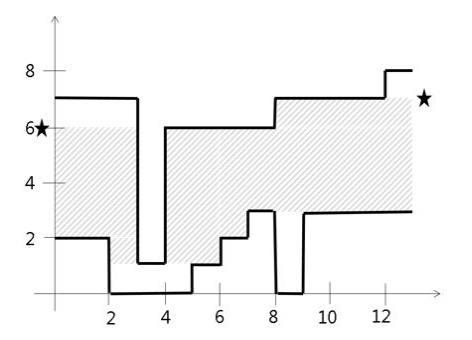
\includegraphics[scale=0.5]{r2_n3.png}

\vspace{3mm}


드론이 움직일 수 있는 경로는 아마도 여러가지가 있을 것이다.

드론이 동굴을 탐험하는 것을 무한히 반복해서 모든 가능한 방법으로 움직인 궤적을 다 그리면 어떤 영역이 나올 것이다.

위에서 빗금친 영역이 그러한 영역이 될 것이다.

이 영역의 면적을 계산하는 프로그램을 작성하라.

(드론은 천정이나 바닥에 무한히 가까이 날 수 있으므로 면적을 계산하는 목적으로는 천정이나 바닥에 붙어서 날수 있는 것으로 생각해도 동일하다.)


\vspace{3mm}

- 제한시간: 전체 테스트 케이스는 30개 이하이며, 전체 수행 시간은 1초 이내. (Java 2초 이내)

    제한 시간을 초과하면 제출한 소스코드의 프로그램이 즉시 종료되며,

    그때까지 수행한 결과에서 테스트 케이스를 1개 그룹 이상 통과하였더라도 점수는 0점이 됩니다.

    그러나, 제한 시간을 초과하더라도 테스트 케이스를 1개 그룹 이상 통과하였다면 '부분 점수(0< 점수< 만점)'를 받을 수 있으며,

    이를 위해서는, C / C++ 에서 "printf 함수" 사용할 경우, 프로그램 시작부분에서 "setbuf(stdout, NULL);"를 한번만 사용하십시오.

    C++에서는 "setbuf(stdout, NULL);"와 "printf 함수" 대신 "cout"를 사용하고, Java에서는 "System.out.printIn"을 사용하시면,

    제한 시간을 초과하더라도 '부분 점수'를 받을 수 있습니다.

    ※ 언어별 기본 제공 소스코드 내용 참고

    만약, 제한 시간을 초과하지 않았는데도 '부분 점수'를 받았다면, 일부 테스트 케이스를 통과하지 못한 경우 입니다.

\vspace{3mm}

\textbf{- 메모리 사용 제한 : heap, global, static 총계 256MB, stack 100MB}
\textbf{- 제출 제한 : 최대 10회 (제출 횟수를 반영하여 순위 결정 → 동점자의 경우 제출 횟수가 적은 사람에게 높은 순위 부여)}

\vspace{5mm}

메모리 사용 제한

\vspace{3mm}

heap, global, static (총계) : 256MB

stack : 100MB

\vspace{5mm}

입력

\vspace{3mm}

입력 파일에는 여러 테스트 케이스가 포함될 수 있다.

파일의 첫째 줄에 테스트 케이스의 개수를 나타내는 자연수 T가 주어지고,

이후 차례로 T 개의 테스트 케이스가 주어진다. $(1 \le T \le 30)$

각 테스트 케이스의 첫 줄에는 동굴의 가로 길이 $L$, 시작 높이 $S$, 끝 높이 $E$가 주어진다.

\vspace{3mm}

다음 줄에 천정을 이루는 가로변들의 개수 $A$가 주어진다. 다음 $A$개의 줄들에,

왼쪽부터 순서대로, 각 가로변의 가로 길이와 높이가 주어진다.

다음 줄에 바닥을 이루는 가로변들의 개수 $B$가 주어진다.

다음 B개의 줄들에, 왼쪽부터 순서대로, 각 가로변의 가로 길이와 높이가 주어진다.

\vspace{3mm}

드론의 시작 위치는 동굴의 왼쪽 끝이고, 최종 위치는 동굴의 오른쪽 끝이다.

드론의 시작 높이와 끝 높이는 동굴의 천정과 바닥 사이이다.

동굴 전체의 길이 L을 포함한 모든 가로 길이는 최대 109인 자연수이다.

모든 높이는 절대값이 최대 109인 정수이다.

동굴의 천정은 동굴의 바닥과 단 한 점에서도 만나지 않는다. $1 \le A, B \le 100,000$이다.

\vspace{3mm}

- 점수 : 각 제출에서 취득한 점수 중에서 최대 점수 (만점200점)

    주어지는 테스트 케이스 데이터들의 그룹은 아래와 같으며,

    각 그룹의 테스트 케이스를 모두 맞추었을 때 해당되는 부분 점수를 받을 수 있다.

    ㆍ 그룹 1 (34점) : 이 그룹의 테스트 케이스에서는 $L \le 1,000, 1 \le A, B \le 100$이고 모든 가로변의 길이와 높이의 절대값은 20이하이다.

    ㆍ 그룹 2 (54점) : 이 그룹의 테스트 케이스에서는 $1 \le A, B \le 100$이다.

    ㆍ 그룹 3 (112점) : 이 그룹의 테스트 케이스에서는 원래의 조건 외에는 다른 제약조건이 없다.

\vspace{5mm}

출력

\vspace{3mm}

각 테스트 케이스의 답을 순서대로 표준출력으로 출력하여야 하며,

각 테스트 케이스마다 첫 줄에는 “Case \#C”를 출력하여야 한다. 이때 C는 테스트 케이스의 번호이다.

다음 줄에 계산된 면적을 정수로 출력한다.

\vspace{5mm}

입출력예

\vspace{3mm}

입력

\vspace{3mm}

1

13 6 7

5

3 7

1 1

4 6

4 7

1 8

7

2 2

3 0

1 1

1 2

1 3

1 0

4 3

\vspace{5mm}

출력

\vspace{3mm}

Case \#1

50
\end{document}
